%%% LaTeX Template
%%% This template can be used for both articles and reports.
%%%
%%% Copyright: http://www.howtotex.com/
%%% Date: February 2011

%%% Preamble
\documentclass[paper=a4, fontsize=11pt]{scrartcl}	% Article class of KOMA-script with 11pt font and a4 format

\usepackage[english]{babel}																% English language/hyphenation
\usepackage[protrusion=true,expansion=true]{microtype}									% Better typography
\usepackage[pdftex]{graphicx}															% Enable pdflatex
%\usepackage{color,transparent}															% If you use color and/or transparency
\usepackage[hang, small,labelfont=bf,up,textfont=it,up]{caption}						% Custom captions under/above floats
\usepackage{epstopdf}																	% Converts .eps to .pdf
\usepackage{subfig}																		% Subfigures
\usepackage{booktabs}																	% Nicer tables

\usepackage{graphicx}
%%% Replace the indent with a newline.
\usepackage{parskip}
%\usepackage{fullpage}

%%% Advanced verbatim environment
\usepackage{verbatim}
\usepackage{fancyvrb}
\graphicspath{{./images/}}
\DefineShortVerb{\|}								% delimiter to display inline verbatim text


%%% Custom sectioning (sectsty package)
\usepackage{sectsty}								% Custom sectioning (see below)
\allsectionsfont{%									% Change font of al section commands
	\usefont{OT1}{bch}{b}{n}%					% bch-b-n: CharterBT-Bold font
%	\hspace{15pt}%									% Uncomment for indentation
	}

\sectionfont{%										% Change font of \section command
	\usefont{OT1}{bch}{b}{n}%					% bch-b-n: CharterBT-Bold font
	\sectionrule{0pt}{0pt}{-5pt}{0.8pt}%	% Horizontal rule below section
	}


%%% Custom headers/footers (fancyhdr package)
\usepackage{fancyhdr}
\pagestyle{fancyplain}
\fancyhead{}														% No page header
\fancyfoot[C]{\thepage}										% Pagenumbering at center of footer
\fancyfoot[R]{\small \texttt{Peter Maynard}}	% You can remove/edit this line 
\renewcommand{\headrulewidth}{0pt}				% Remove header underlines
\renewcommand{\footrulewidth}{0pt}				% Remove footer underlines
\setlength{\headheight}{13.6pt}


%%% Title	
\title{ \vspace{-1in} 	\usefont{OT1}{bch}{b}{n}
		\huge \strut Industrial Placement Report \strut \\
		\Large \bfseries \strut There is no spoon. \strut
}
\author{ 									\usefont{OT1}{bch}{m}{n}
        Peter Maynard\\		\usefont{OT1}{bch}{m}{n}
        University of Aberystwyth\\	\usefont{OT1}{bch}{m}{n}
        Computer Science\\
        \texttt{pem9@aber.ac.uk}
}
\date{}

%%% Begin document
\begin{document}
\maketitle
\begin{abstract}
This report will explain in detail what I did during my twelve month industrial placement at Draig Technology. It will detail the organisational environment as well as the technical and non-technical environment in which I worked. It will evaluate my activities and experiences I gained during my time there.
\end{abstract}

\clearpage
\tableofcontents
\clearpage

\section{Organisational Environment}
Draig Technology Limited\cite{draig} is a small software company located in Bangor north Wales, it was founded in 1999, by Richard Sheppard who is the managing director.  Since then it has worked on a variety of different projects ranging from web design, Microsoft Share Point\cite{sharepoint}, network management and other bespoke software packages. For the last few years Draig has specialised in being the leading supplier in the UK for Customer Relationship Management (CRM) and Billing solutions in the energy sector for small to medium sized companies. Draig is a Microsoft certified business and has been financially stable for over 10 years. 

The company is split into two teams. The first is the support team, which provides support for the Draig Billing System (DBS).  This consists of triaging client issues, testing new versions of DBS and coordinating with clients when an update or patch is to be applied. The second team is development, which mainly works on DBS, as well as providing support for client issues.

The two teams are physically separate, with the support team and administration staff in a smaller upstairs office, which consists of an office manager, two project managers and the managing director. The development team is located downstairs in a larger office. There are around eight members of the development team including another intern and project manager. During my twelve month employment, a few members of the development team left the company, with new members replacing them. This also included contractors, who were in employment for around four to five weeks.

I was employed in the support team as technical support. When I started there were three teams, Support, Testing and Development. The support team consisted of me and my manager, testing also had the same amount of members. I worked closely with both testing and support until around seven months into my employment, when the leader of the testing team left the company. The remaining members of testing were merged into support. Figure \ref{fig:current_structure} shows the current company structure and Figure \ref{fig:original_structure} shows the original structure.

\begin{figure}[htb]
\centering
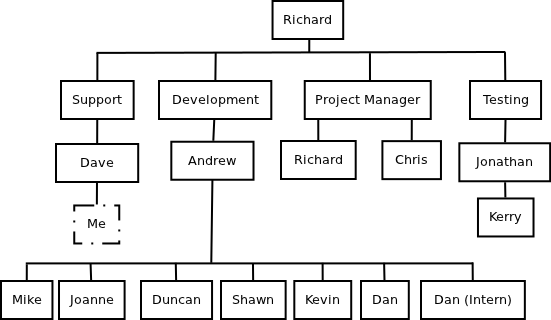
\includegraphics[width=0.8\textwidth]{OriginalStructure}
\caption{Original company structure}
\label{fig:original_structure}
\end{figure}

\begin{figure}[htb]
\centering
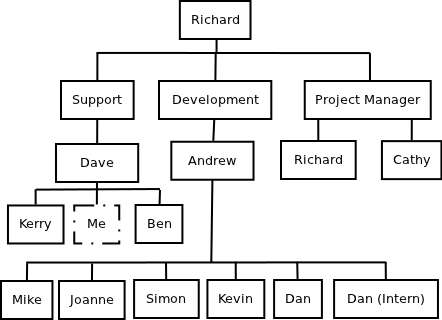
\includegraphics[width=0.8\textwidth]{CurrentStructure}
\caption{Current company structure}
\label{fig:current_structure}
\end{figure}

For each of the teams there is a team manager who reports to the managing director.  Aside from the two support and development teams, there are client project managers which work closely with one or more clients, they ensure that their respective projects are on track and have been given the resources they require.

Being in the support team meant that I reported to the manger of the team, who was in charge of my tasks and made sure targets were met. Although not all of my tasks were support related, due to Draig being a small company, many of my tasks would come from the managing director and other team leaders. When there was a testing team, the team leader would often request me to assist him with his activities.

During the last few months of my employment, Draig hired another employee to work in the support team. He will be taking over my position when I leave, he reports to the support manager, and I was his main point of entry to the company and acting as his mentor.

\section{Technical and Application Environments}
Draig have around three main servers. All the servers are Dell Power edge, with the main server being an Intel Dual Core Xeon, 32GB RAM. The workstations are split up into two types, development and management. Development machines consists of a Dell XPS, with an Intel Quad Core, 8GB RAM and 1TB HDD. Management machines varied from mid range desktops to laptops, the majority were laptops with 4GB RAM and 500GB-1TB HDD. Support use the same specification machines as development. All machines have dual monitors, of excellent quality. We were encouraged to store our documentation and scripts on the network drive, which was a Windows NTFS share, running on the main server. Occasionally this device would run out of space, bringing down the whole issue tracking system. Which from a support and business perspective this is not a good thing as this is client facing. From my experience working at Draig, I would separate storage and issue tracking to another physical or virtual machine, so that when the network storage becomes full, the issue tracking service would not fall over. Though I believe this issue has been resolved, and the cause was down to a dodgy backup script. 

The servers are located downstairs with the development team. The network between the two offices is part of the building, and is managed by a building wide network. This is also where external WAN access is provided\cite{fiberspeed}. Networking within the two offices is managed internally. This is accomplished by running DHCP and DNS services on the main server. Physical machines are linked together with Ethernet and have a star topology. Each office has a dedicated 24port Switch, with WiFi being supported by two wireless access points.

Overall I found that the quality of hardware, helps make a positive effect on work productivity. The ability to perform multiple tasks quickly helps keep me focused. When for example I was working remotely on a clients server, their network was experiencing networking issues, which resulted in a nightmarish time in setting up and configuring their server. Needless to say this was not one of the most productive days I had. 

Draig is an official Microsoft partner, this means that the majority of their software which they use are Microsoft based. Draig have a main domain server which is used for external VPN access and user administration. The email service is outsourced to a company called simply mail solutions\cite{simplymail}, which provide web and Microsoft Exchange access. All of the workstations are configured to use outlook 2007/12 and the exchange server. Development is done using Visual Studio 2005/12\cite{VS}. For code management and client support, e.g. reporting software issues, we use Team Foundation Server (TFS)\cite{TFS} which is an extension to Visual Studio. TFS provides clients with a web interface to report and track issues, as well as developers with version control. The advantage of this is that developers can log their work directly on the issue which was raised by the client. 

All of the machines run Windows Server 2008 RC 2 aside from the main server which runs Windows Server 2003, and some of the machines which are used solely for administrative tasks  run Windows XP. For development, due to Microsoft CRM 4.0\cite{CRM} and Visual Basic 6 restrictions, we are forced to use virtual machines which contain CRM 4.0 and some DBS subsystems. DBS was originally built in Microsoft Access, and has since been upgraded to use more enterprise level software, though some of the original code still exists inside Access, this is where Visual Basic 6 comes in. Draig is actively moving away from VB6 and Access.

Draig use Microsoft Share point as their main form of content storage and sharing. The share point site has sections for each team as well as each client.  This is used to store information such as documentation for DBS and project plans for clients. Microsoft Project\cite{project} is used to manage each team, and future client releases. All of the documentation are written in Microsoft Office 2012/07.

For time management Draig use an in house system called ETHEL (Escape from time sheet hell). When an employee works on a project they must make sure to record it in ETHEL, this also gets linked to the TFS issue number.

I've found using Microsoft based software a bit strange to get used to, as it tends to do things the long way round. I also find it provides me with less customizability and features than other alternative software. For example, every week we have a report which is complied using data from TFS, the issue tracking system, and a word template. This requires the data to be manually placed in the Word template. Given some time it would be possible to completely automate this using free open source software such as LaTeX and bash and the results would be identical, if not better. I can see the advantages of using industry standard software as this would be a positive for Draig. I did bring this idea forward, but due to work load and deadlines nothing more was done with this.

For testing we run virtual machines (VM) on the main server, for each client we run a Factory Acceptance Testing (FAT) VM. This is where the majority of testing is carried out, before it is deployed to the client's User Acceptance Testing (UAT) server. Then from UAT the system is deployed to the Live server, after it has passed client testing. Draig use an agile development life cycle. 

From my experience with this process, I have found that problems can happen when taking a back up from live and restoring it on a UAT/FAT server. Due to the way that DBS manages its configuration, when backing up the database it will also backup the absolute URL of the live server. So when the back up is restored the UAT/FAT system will attempt to establish communications to the live server. As you can imagine having a test server communicating with the Live server is not ideal, as users will believe they are editing data on the test server, when in actual fact changes will be made to live data.

\subsection{Application Environment}
\begin{figure}[htb]
\centering
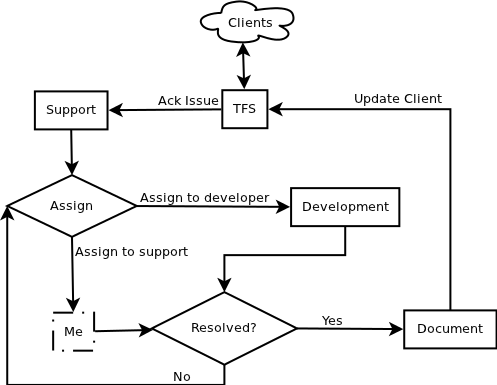
\includegraphics[width=0.8\textwidth]{DataFlow}
\caption{Data Flow of the service desk}
\label{fig:data_flow}
\end{figure}
Due to working in the support team, I get to utilize all software and systems within the company.
With the majority of my time spent working with the issue tracking system, i.e Visual Studio's Team Foundation Server. When an issue is reported I pick it up from the list and begin my investigation, this would normally involve me loading up Microsoft SQL Server Management Studio\cite{SSMS} (SSMS) and identifying the issue on the Live or FAT server. If this is the first time this issue is reported I would record any steps taken to resolve the issue, and store the script on the network share. Once the issue has been resolved, I update TFS with my actions, and set the issue to 'Awaits Live Confirmation'. This notifies the client that action has been taken, they test it and if all goes well the ticket is closed.
If it is an important issue then it is normal to personally contact the client, and update them when progress has been made. Figure~\ref{fig:data_flow} shows the flow data within the compnay from the service desk's perspective.

For issues which require a code change, I would develop a fix using my local version of DBS. Once I believe it's working I get it checked by one of the senior developers. If it passes the development check the code will be committed to the version control system. I will then deploy it to the FAT server, where it will then be checked by one of the members of the testing team. In some cases this would be me. After it has passed all the testing, the fix may be applied to the live server.

\section{Activities Undertaken}
When I first started working at Draig, I was placed downstairs with the development team.  For the first month I was tasked with learning how DBS works and how to use it.  This also involved how to set-up and get DBS working on my local machine. This meant compiling DBS from source and get it configured with Microsoft CRM running in a virtual machine. After I had become familiar with DBS I was assigned to the bench testing project. Bench testing is split into four main categorises: 

\begin{enumerate}
	\item Input: The entrance criteria or deliverables needed to perform work, 
	\item Procedures to do: The tasks or processes that will transform the input into the output, 
	\item Procedures to check: The processes that determine that the output meets the standards, 
	\item Output: The exit criteria or deliverables produced from the workbench. 
\end{enumerate}


I had to create scripts which would generate usable data. Datasets were based on the number of supplies, ranging from 10k, 25k and 50k. Once a billing run was tested on 50k I then continued to run the duplication scripts until the system failed or we hit 2million supplies. To create the datasets I used original data and duplicated it, I had to make sure that the data I was duplicating was free from errors, because if a customer and supply did not bill then this will provide an inaccurate result. Duplicating the data takes about three days of continues processing.

This is the first official stress testing done on the DBS system, and the results were positive. Later on in the year the results were sent to one the clients and they requested the data creation scripts, in order to recreate me results. During the course of their testing I provided support and assistance. In the end they were happy with the results.

Also following on from bench testing, I was asked to write a small test harness for stress testing the system, this would generate and destroy a statement for a customer 'n' amount of times. This stress testing tool was designed as part of a larger performance suite, which was being developed by the development team downstairs.  Although this application was not used, it provided me with vital information about DBS, and helped further my understanding of the DBS Web Service.

The second of the tasks was to research and create an automatic user interface (UI) testing scripts. For this I used WatiN\cite{WatiN}, which uses Document Object Model (DOM, HTML) and Unit Testing built into Visual Studio. The initial stages where successful but after the loss of the lead testing manager this project was not followed up.

During my time at Draig I found that many projects and activities that I undertook were not completed, and that the initial development stage was the farthest the projects would get to. I understand that this a result of a small business. The positive of this is that I got to work on many different different projects and activates. 

Half way though the bench testing and UI automation projects, I was moved up stairs to the support department. Which meant I now report to to the lead support manager and not development. As well as my original projects, my role in the department was to provide technical support and assistance with the service desk. Working on the service desk meant that I had to reply to emails from clients and assist in managing the phones. When a client phoned up with an issue, I would have to make sure that it gets logged into our system. If the issue is urgent, I would inform the manager of the development team, and hope a developer starts working on it. In other cases if the call was not urgent, then they would be placed on the review list, where a member of the support team would meet with the development team leader, and they would assign the issues to members of  support and development.

During the first five months on the service desk I was tasked with identifying support activities, this is an issue which could be resolved with little technical information. This meant that when a support activity is identified, I would work with one of the developers to solve the issue. This would involve shadowing the developer when they are fixing the issue, and making notes so that I would be able to do it again on my own. Once I was able to fix the issue with out any developer assistance, I would begin working on a automatic script which would be able to identify any other instances and fix any future issues. The script would then be reviewed by one of the developers and put to use on the service desk.

For the first seven months I was working with the testing department, this would involve testing the latest changes of the software on our FAT server, before it is passed to UAT. During this time I learned some of the key systems of DBS inside out, this was a vital and useful skill because the developers downstairs were not always available for support of the FAT server. This would mean than due to a misconfiguration or a bug FAT would not work, or provide the correct output. To get around the fact that there was no technical support, me and the other testing personal had to learn how to repair the system. Form me this was good, as I would learn about the system and how to repair it, but from the testing prospective this was not good, as it does not provide a constant or solid framework to test the system. I also had to create some of the test data, as the FAT system would use a backup of the Live data, and in some cases the exact data was not found. After the testing manager left, I did less testing, as this is now done by my manager.

Four months into my employment I was assigned a project which was originally maintained by the previous intern. This is an application which will provide administrative actions over DBS without having to have a technical background. This is designed to be sent over email and used by the clients. So some of the key features of the application was that it had to be small and have the ability to configure it remotely. It will also provide the user with a list of reports which can be run, these reports will list any identifiable issue, which was discovered either by the client or from internal testing. It also provides the user with a potential fix for the issue. The second feature of the admin utility is that it will provide the user with access to the automatic scripts which I wrote during my time on the server desk. In most cases the admin utility it's self would be able to repair the issues reported.

This application was in use by the service desk before I left and was about to be released to the clients. After I had completed my twelve month employment, I as asked if I wanted to work on contract to implement a few extra features to the admin utility which is currently in testing.

Another aspect of my work was to deploy DBS remotely onto client's servers. This was an area I wished to pursue, and as such I brought it up in on of my reviews.  After that I was allowed to  shadow deployment and software updates, making notes and performing them on our FAT server and on my local virtual machines. This also involved updating or creating documentation regarding server deployments, as much of the documentation was either out of date or incomplete. I gained a lot of experience working with Windows server and Visual Basic 6, mainly DLL registration, incidentally this is a nightmare. Over the course of my employment I was given more responsibilities in the way of deployments. Despite my accidental mistake of editing the Live server's files instead of the UAT server and causing system downtime.

The last two months of my employment at Draig, I was asked to bring a new employee up to speed, to essentially replace me. This was an interesting experience, where I was being shadowed during my day to day work. This also meant explaining how DBS works and what is required of my position.

\section{Critical Evaluation}

\subsection{Technical}
I found even though I was an intern, Draig believed in my abilities and allowed me to work on my own with out supervision. For example, when I was developing the bench testing scripts this was my first project, and as such I did not have much experience with DBS. Despite this, my superiors were happy to use my results as an official benchmark of the system, and provide clients with my scripts. All this without having a code walk though by a senior developer. This was nice, but I think I would have been happier if my methods were approved before accepting my results. Though this has given me a lot more confidence in my work than I had before, as they were more than happy with what I had accomplished.

From my experience, I often found that much of the testing was not done, for example once the code had been written and confirmed working by one of the developers this might not get any further testing, until it's tested by the client on their UAT server. Though this is not always the case with large patches or releases. This is the opposite of what I was taught in my testing module, I believe this is because Draig is a small company still working out what process work well with clients. The good news is they are always looking for ways to improve. As towards the end of my employment a more stable testing protocol was beginning to be implemented.  I've also learnt that testing every aspect of a system is not the best approach, there is a finer trade off between testing and time developing, than I had previously thought.

With Draig being a Microsoft based company, I had hoped to learn skills relating to Microsoft. In this respect I did. Draig's language of choice is Visual Basic, which in turn uses the Visual Studio IDE. After using Visual Studio for developing software and issue tracking, I have learnt how to utilize many of the advanced features of the software, as well as how projects are stored and managed within TFS. I've gained experience on how to access the low levels of the issue tracking  database to manually generate reports. I've deployed VB6 code and forced Dynamic Linked Libraries (DLL) to register successfully. This is something I do not wish to do again, but gives me a great insight in to how Window based systems work, and how to develop on Windows using their native development software. Working in Windows is a completely different feeling than working in a GNU/Linux environment and has changed the way in which I look at both of them.

An area which I have gained experience with is managing Windows server 2008 RC 2. I am able to configure the basic requirements of a Windows server so that it is able to correctly run a full version of DBS. This involves configuring all supplicant Windows services and ensuring the correct dependences are installed. I also spent some time managing virtual machines running both Hyper-V\cite{hyperv} and Virtual Box\cite{vbox}. This is a something which I requested to do and really enjoyed.

Due to the nature of DBS I gained massive experience with Microsoft SQL Server. As all data is stored inside the SQL database, this needed to be backed up and restored on many occasions. Also a lot of the support issues can be resolved by looking at the database and seeing what exists or does not. This meant that I spent a lot of time using SQL Server Management Studio and as such found it to be a far more useful application than I thought. Before I started working for Draig I saw not much use to a Graphical User Interface (GUI) SQL IDE, as I spent all of my time using a Command Line Interface (CLI). I also believe I have picked up some backing up habits, such as naming convention and making sure backs up actually works. In all I believe working with SQL servers has been an excellent experience as I have gained a greater incite into the way businesses handle large datasets. 

Draig use a CRM system called Microsoft CRM 4.0, this provides the end user with a clear and easy to use interface to customer information. Draig's Billing System, integrates seamlessly into Microsoft CRM. This means that for technical support a lot of the issues require us to look a the underlying CRM system. I gained a lot of experience with CRM. I believe I would never get such a experience with any other company, and have found it to be interesting and rewarding. The knowledge I had learned from working with Microsoft CRM will provide me with an advantage in my future career. 

\subsection{Non-technical}
Some of the first things which happened quite frequently, which I had to get used to was the amount of meetings we had, often a lot of information would be exchanged, and I would be assigned tasks from the results of the discussions. Once I got the hang of meetings I was able to identify my required deliverables with out any problems. I believe even though this was not hard, it was an excellent learning experience. Working with other people each with their own list of activities, and deadlines. I often found that I would be working on more than one thing at once, which meant I would have to leave one project to work on another, this would change depending on other people's priorities and constraints. Making sure that my time management coincided with other members of the team, was an interesting experience, I would have to make sure that if I helped person X that I still had enough time to complete project Y.

Phone etiquette I found a little harder to get right, I would find that I'd forget to ask who was calling, or the full details of the call. Also trying to pick out the core components of a call took some time to get to grips with. I found email etiquette to be a lot easier than phone, the main things to remember were to make sure the font size and type where within the company standard. Also ensuring that each email had a standard business signature. I could understand why this was important, as the majority of businesses communication with clients are via email, and showing a conformed standard of communication is essential. After a while I started to become accustom to how clients reacted to a situation, and who to and who not to 'cc'. This is vital in the current age we live in, being able to construct quality emails is one of the most important skill that I have learned during my time at Draig.

Documentation was one of my main activities, due to the fact that I would be leaving, I needed to make sure that my replacement would have all the information required to continue my position. All of the documentation should follow the companies document guidelines, just like the email. I often found that a lot of the original documentation was simple notes made by the developer when they were performing the action. This meant that for someone like me who had never done the procedure , there were large sections which were missing and made no sense. This gave me the chance to update and improve the document for future use. Though most of the time I was creating the original documentation. I believe I have greatly improved my ability to manage and maintain documentation, if not my typing speed and accuracy has greatly improved. 

Reports which get sent to the clients, have to be correct and of a certain quality. This gets checked by the heads of support, development, and the project manger before the report is sent out to the client. This had to be accurate to insure we are giving the client a clear and understandable picture   of the service desk. I found this to be a tedious job, trying to work out which number was wrong and the reason why, most cases the issues would be down to the process used to query the results from TFS, the issue tracking system. I believe that I have a better ability to identify mistakes and problems with documents that I create after this experience.

\subsection{Overall Evaluation}
Overall I feel that I have learnt more soft skills than technical skills, this is not a bad thing as these skills are essential for any position I latter apply for. I have found the experience to be interesting and enlightening, whilst working with Draig I was able to gain experience working in a small software development company, during my time there I was never treated differently to other employees.

After my industrial placement I had hoped that I would know what area I wanted specialise in after my degree. My reasons for applying for Draig's software development position, was so that I could gain experience working as a software developer, rather than applying for network/server engineer positions. Due to being assigned to the support team, I did not work solely on software development. I did a mix of the two as well as much more. Which whilst it was a great experience, it did not help me work out what area to specialise in.

\begin{thebibliography}{9}

\bibitem{draig}Draig Website, \emph{http://www.draig.co.uk}
\bibitem{sharepoint}Sharepoint, \emph{http://sharepoint.microsoft.com}
\bibitem{fiberspeed}Parc Menai Internet Provider, \emph{http://www.nwcolo.co.uk/articles/connectivityarticles/fibrespeed}
\bibitem{simplymail}Simply Mail Solutions, \emph{http://www.simplymailsolutions.com}
\bibitem{VS}Visual Studio, \emph{http://www.microsoft.com/visualstudio}
\bibitem{TFS}Team Foundation Server, \emph{http://msdn.microsoft.com/en-us/vstudio/ff637362.aspx}
\bibitem{CRM}Microsoft CRM, \emph{http://crm.dynamics.com/en-gb/home}
\bibitem{project}Microsoft Project, \emph{http://www.microsoft.com/project}
\bibitem{SSMS}SQL Server Managment Studio, \emph{http://www.microsoft.com/sqlserver/en/us/solutions-technologies/database-management.aspx}
\bibitem{WatiN} WatiN, \emph{http://watin.org}
\bibitem{hyperv}Hyper-V, \emph{www.microsoft.com/hyper-v}
\bibitem{vbox}Virtual Box, \emph{https://www.virtualbox.org}

\end{thebibliography}

\end{document}
